\documentclass[11pt,a4paper]{article}
\usepackage[T1]{fontenc}
\usepackage[utf8]{inputenc}
\usepackage[french]{babel}
\usepackage{lmodern}
\usepackage{microtype}
\usepackage[margin=2.3cm]{geometry}
\usepackage{graphicx}
\usepackage{booktabs}
\usepackage{float}
\usepackage{caption}
\usepackage{csquotes}
\usepackage[style=numeric-comp,sorting=none,backend=biber,maxbibnames=4]{biblatex}
\usepackage[hidelinks]{hyperref}
\usepackage[french]{cleveref}
\addbibresource{../../latex/references.bib}
\graphicspath{{../results/figures/}{../../vosges/results/figures/}}
\captionsetup{font=small,labelfont=bf}

\title{Bande L (NISAR) contre bande C (Sentinel-1) pour la détection des coupes rases\\
dans le Morvan, selon la méthode du guide de l'Irstea\\[0.4em]
\large Réplication de l'étude de faisabilité des Vosges}
\author{Mamadou Galy Diallo}
\date{Novembre 2026}

\begin{document}
\maketitle

\begin{abstract}
\noindent
Cette étude réplique dans le Morvan (sylvo-écorégion G23) l'étude de faisabilité menée dans les Vosges, qui
comparait la bande L de NISAR et la bande C de Sentinel-1 pour détecter les coupes rases. Elle suit la méthode du
guide de l'Irstea. Appliquée telle quelle à Sentinel-2 en intra-saison, cette méthode détecte 8,7~\% de la forêt,
essentiellement de la sénescence de feuillus. Une référence qualifiée, puis contrôlée par photo-interprétation,
retient 7 coupes de peuplement fermé (15,4~ha) dans une fenêtre de $20\times20$~km couverte, à géométrie égale,
par deux géométries NISAR et deux orbites Sentinel-1.

La forêt reste cohérente en bande L (0,5--0,7 à 12~jours) mais pas en bande C (0,25--0,36, plancher de
l'estimateur). En géométrie descendante, la cohérence L sépare les coupes de la forêt (AUC 0,81 contre 0,52 en C).
En rétrodiffusion croisée, les AUC sont proches (0,80--0,83 en L, 0,73--0,83 en C), mais le contraste est plus
marqué en bande L (d de Cohen 1,9--2,1 contre 1,0--1,6). Transposée au radar, la méthode du guide fonctionne
nettement mieux en bande L (kappa 0,41, 5 coupes sur 7) qu'en bande C (kappa 0,08--0,16, 2 à 3 coupes), sans
atteindre l'objectif de 10~\% d'erreur. Les fausses alertes de la bande C se concentrent sur des parcelles déjà
ouvertes, où évolue la végétation basse.

La qualité de la référence optique conditionne les résultats : avec la référence automatique, aucune bande ne
sépare les coupes (AUC 0,51--0,56).
\end{abstract}

\tableofcontents
\newpage

%=====================================================================
\section{Contexte et objectif}

Les bandes radar de grande longueur d'onde (L et P) sont réputées mieux adaptées que la bande C au suivi des
forêts. Une première étude, dans les Vosges, a comparé NISAR (bande L, produits
de niveau~2 générés par ISCE3~\cite{isce3}) et Sentinel-1 (bande C~\cite{torres2012sentinel1}) sur une coupe rase
de 2,4~ha. La bande L y séparait presque parfaitement la coupe de la forêt en cohérence interférométrique
(AUC 0,995 contre 0,72 en bande C), mais son avantage en rétrodiffusion dépendait de la géométrie d'acquisition.
Cette étude avait deux limites : \textbf{une seule coupe} et \textbf{une seule orbite Sentinel-1}.

La présente réplication lève ces deux limites et s'appuie sur une méthode opérationnelle française : le guide
méthodologique de détection des coupes rases de l'Irstea (UMR TETIS)~\cite{ose2015guide}, établi pour le ministère
de l'Agriculture sur la sylvo-écorégion G23 \enquote{Morvan et Autunois}. Ce guide sert à la fois :
\begin{enumerate}
\item de \textbf{référence optique} : sa méthode est appliquée à Sentinel-2 sur toute la G23, puis contrôlée par
  photo-interprétation ;
\item de \textbf{norme d'évaluation} : sa méthode de seuillage est transposée aux images de changement radar et
  évaluée avec sa matrice de confusion en surface et ses objectifs ($\leq 10$~\% d'omission et de commission).
\end{enumerate}
La bande L sera assurée en Europe par la mission Copernicus ROSE-L~\cite{esa2020rosel} ; la chaîne développée ici
lui est directement transposable.

\paragraph{Question.} \emph{Sur plusieurs coupes rases du Morvan (juin--novembre 2026), et à géométrie égale dans
les deux directions de visée, la bande L de NISAR distingue-t-elle mieux les coupes de la forêt intacte que la
bande C de Sentinel-1 ? Et une méthode opérationnelle comme celle du guide est-elle transposable au radar ?}

\paragraph{Hypothèses}, reprises des Vosges :
\begin{description}
\item[H1] La cohérence de la forêt intacte est plus élevée en bande L qu'en bande C.
\item[H2] La perte de cohérence due à la coupe est donc mieux détectée en bande L.
\item[H3] La baisse de rétrodiffusion après la coupe est plus forte en bande L, la bande C saturant sur forêt
  dense~\cite{imhoff1995saturation,joshi2015mapping}.
\item[H4] La polarisation croisée est l'indicateur de rétrodiffusion le plus sensible.
\end{description}

%=====================================================================
\section{Zone d'étude et données}

\subsection{La sylvo-écorégion G23 « Morvan et Autunois »}

La zone d'étude est celle du guide méthodologique de l'Irstea~\cite{ose2015guide} : la sylvo-écorégion
G23~\cite{ign2011ser}, massif de moyenne montagne (environ 200 à 900~m) de 3\,011~km² à cheval sur la Nièvre, l'Yonne, la
Côte-d'Or et la Saône-et-Loire. La forêt y couvre environ la moitié du territoire (52~\% d'après la BD Forêt). Le massif est connu pour ses
plantations de résineux, surtout de douglas, qui sont exploitées par coupes rases et remplacent progressivement la
forêt feuillue (chênaie, hêtraie). La BD Forêt V2~\cite{ign2024bdforet}, lue par le service WFS de la
Géoplateforme, donne 13\,494 polygones de forêt. En ne gardant que les forêts à couvert arboré et les peupleraies
(la classe FF0, \enquote{forêt fermée sans couvert}, correspond à des coupes anciennes), on obtient environ
157\,800~ha : 89\,750~ha de feuillus, 49\,400~ha de résineux et 18\,600~ha de forêts mixtes.

\subsection{Données}

\begin{table}[htbp]
\centering\small
\caption{Données utilisées sur le Morvan (juin--novembre 2026).}
\label{tab-data}
\begin{tabular}{p{2.7cm}p{5.4cm}p{6.7cm}}
\toprule
Capteur & Produits & Détails \\
\midrule
NISAR (L, 1,26~GHz) & L2 GCOV ($\gamma^0$ HH, HV, RTC) et GUNW (cohérence HH à 20~m), produits par
ISCE3~\cite{isce3} & 2 géométries couvrant la fenêtre radar : A173~F25 (montante) et D66~F65 (descendante). Paires
de 12 à 24~jours. \\
Sentinel-1 (C, 5,4~GHz) & IW SLC, VV+VH, traités avec SNAP~\cite{snap} & Orbites A59 (IW3) et D37 (IW2), 3 bursts
chacune. 15 dates à 12~jours par orbite, du 01/06 au 18/11/2026, presque toutes de S1D. \\
Sentinel-2~\cite{drusch2012sentinel2} & L2A, NDVI et SWIR & Référence : méthode du guide sur toute la G23 (tuiles
31TEM, 31TEN, 31TFM, 31TFN) et photo-interprétation. \\
IGN & Contour G23, BD Forêt V2 & Masque forêt et groupes (feuillus, résineux, mixtes). \\
\bottomrule
\end{tabular}
\end{table}

Comme dans les Vosges, les volumes téléchargés sont réduits : les produits NISAR sont lus à distance par blocs
HDF5, et seuls les fichiers de la sous-fauchée utile sont extraits des archives Sentinel-1.

%=====================================================================
\section{Méthode}

\subsection{La méthode du guide}

Le guide~\cite{ose2015guide} détecte les coupes rases en six étapes : NDVI de deux images d'été, différence
$\Delta$NDVI, masques zone d'étude et forêt, seuillage statistique dans la forêt, tamisage à 1~ha et évaluation par
matrice de confusion en surface. Le seuillage utilise la moyenne $m$ et l'écart-type $\sigma$ de $\Delta$NDVI
dans la forêt, avec trois degrés de certitude :
\begin{center}\small
\begin{tabular}{ll}
\toprule
Degré & Intervalle \\
\midrule
1 (faible) & $[m-2\sigma, m-\sigma[$ \\
2 (moyen) & $[m-3\sigma, m-2\sigma[$ \\
3 (fort) & $< m-3\sigma$ \\
\bottomrule
\end{tabular}
\end{center}
Ses spécifications sont une unité minimale de 1~ha et des erreurs d'omission et de commission $\leq 10$~\% en
surface. Le module \texttt{nisar\_s1.guide\_cr} implémente ces étapes pour n'importe quelle image de changement
($\Delta$NDVI, $\Delta\gamma^0$, baisse de cohérence), avec le sens du changement en paramètre.

\subsection{Référence optique}

\paragraph{Guide appliqué à Sentinel-2.} Pour chaque tuile, le NDVI est la médiane des 3 dates les plus claires de
deux fenêtres : \enquote{avant} (15/06--08/07/2026) et \enquote{après} (15/09--16/10/2026). Les seuils du guide
sont calculés dans la forêt de G23.

\paragraph{Référence qualifiée.} Le guide ne retient que les parcelles \enquote{passées d'un état boisé à un état
sol nu}. La référence est donc : degré~3, NDVI avant $\geq 0{,}70$, NDVI après $\leq 0{,}65$, puis tamisage à
1~ha.

\paragraph{Photo-interprétation.} Comme le recommande le guide (section 3.9.1), la référence est contrôlée
visuellement : couleurs vraies avant et après, et fausses couleurs SWIR / PIR / rouge après, où le sol nu et les
rémanents apparaissent rose-magenta. Chaque objet reçoit un verdict : coupe certaine, probable ou sans sol nu.

\paragraph{Test \enquote{forêt avant}.} Une coupe rase est la perte d'un peuplement fermé. La réflectance SWIR
(B11) de juillet dans l'objet est comparée à celle d'un anneau de forêt de 100 à 400~m : l'objet était un
peuplement fermé si sa B11 ne dépasse pas le 90\textsuperscript{e} centile de l'anneau.

\subsection{Fenêtre radar}

Le traitement Sentinel-1 se limite à 3 bursts d'une seule sous-fauchée (mémoire vive). Les fenêtres de
$20\times20$~km ont été classées selon la surface de coupes de référence, puis contrôlées dans les catalogues ASF :
une orbite Sentinel-1 montante et une descendante, chacune dans une seule sous-fauchée, et au moins une géométrie
NISAR montante et une descendante. La fenêtre retenue (nord-est de G23) permet, contrairement aux Vosges, la
comparaison \textbf{à géométrie égale dans les deux directions} : A173 (L) contre A59 (C) en montante, D66 (L)
contre D37 (C) en descendante.

\subsection{Traitements radar}

\begin{itemize}
\item \textbf{NISAR} : $\gamma^0$ HH et HV des GCOV (RTC~\cite{small2011flattening}) et cohérence HH des GUNW,
  utilisés tels que livrés par ISCE3 et rééchantillonnés sur la grille Lambert 93 de 20~m.
\item \textbf{Sentinel-1} : mêmes graphes SNAP que pour les Vosges. Pour $\gamma^0$ : calibration,
  Terrain-Flattening et géocodage. Pour la cohérence : fenêtre $10\times3$, phases plate et topographique
  retirées. Les 3 bursts sont raccordés par TOPSAR-Deburst, sans ESD.
\end{itemize}

\subsection{Variables de changement}

Les acquisitions sont classées en \enquote{avant} (01/06--12/07), \enquote{après} (10/09--20/10) et
\enquote{entre} ces deux fenêtres, qui encadrent les fenêtres optiques. Les dates de coupe ne sont pas connues
une à une : les variables sont donc définies pour être indépendantes de la date exacte.
\begin{itemize}
\item $\Delta\gamma^0$ : $\gamma^0$ moyen après $-$ $\gamma^0$ moyen avant (dB, moyennes en puissance linéaire) ;
\item $\gamma^0$ après (dB) ;
\item cohérence minimale sur les paires \enquote{entre} : la paire qui encadre la coupe en fait partie, quelle que
  soit la date de la coupe ;
\item chute de cohérence (cohérence avant $-$ cohérence minimale) et cohérence après.
\end{itemize}

\subsection{Évaluation}

\paragraph{Classes.} La classe \enquote{coupe} est formée des pixels forestiers des coupes de référence. La classe
\enquote{forêt intacte} est la forêt BD Forêt dont $\Delta$NDVI reste dans $m \pm \sigma$ et située à plus de 40~m
de toute détection optique. Les objets écartés par la photo-interprétation et une zone tampon de 40~m sont exclus
des deux classes.

\paragraph{Séparabilité.} Pour chaque variable : AUC (statistique de Mann-Whitney~\cite{hanley1982auc}, exprimée
comme $\max(\mathrm{AUC}, 1-\mathrm{AUC})$), d de Cohen~\cite{cohen1988power} et distance de
Jeffries-Matusita~\cite{swain1978remote}. Les intervalles de confiance à 95~\% sont obtenus par un bootstrap en
grappes~\cite{kunsch1989bootstrap} : on rééchantillonne les coupes entières (et non les pixels, qui sont
corrélés) et des blocs de $5\times5$ pixels de forêt. Avec 7 coupes, ces intervalles sont larges.

\paragraph{Contrôles.} Avant la coupe, coupes et forêt doivent être indiscernables. On le vérifie par le
changement entre deux dates \enquote{avant} et par le niveau de $\gamma^0$ avant la coupe, qui révèle un éventuel
effet du type de peuplement.

\paragraph{Transposition du guide au radar.} Les degrés de certitude $m-k\sigma$ sont calculés sur chaque variable
radar dans la forêt de la fenêtre, puis tamisés à 1~ha. On calcule ensuite la matrice de confusion en surface du
guide contre la référence (omission, commission, kappa) et la part des coupes trouvées (au moins 25~\% de leurs
pixels détectés). On calcule aussi le taux de fausses alertes rapporté à la surface forestière : avec une
référence de quelques hectares, la commission relative du guide est très sensible à quelques hectares de fausses
alertes.

\paragraph{Audit des fausses alertes.} Les plus grandes détections radar hors de toute détection optique sont
photo-interprétées sur une image Sentinel-2 tardive (novembre) : une partie peut être des coupes réalisées après
la fenêtre optique de septembre.

\paragraph{Datation.} Pour chaque coupe de référence et chaque géométrie, la série de $\gamma^0$ en polarisation
croisée est comparée à son niveau d'avant juillet. La coupe est datée entre la dernière acquisition normale et la
première acquisition d'une baisse durable de plus de 2~dB (deux acquisitions consécutives).


%=====================================================================
\section{Résultats}

\subsection{La référence optique}

\paragraph{Le guide appliqué tel quel sur Sentinel-2.} Dans la forêt de G23, les seuils du guide valent
$m=-0{,}040$ et $\sigma=0{,}058$ ($\Delta$NDVI). La méthode produit 3\,349 objets de 1~ha ou plus (13\,600~ha),
soit \textbf{8,7~\% de la forêt en deux mois et demi}, alors que le taux de coupe rase est de l'ordre de
1~\% par an. Les détections sont surtout des feuillus, qui jaunissent dès septembre
(\cref{fig-s2-overview}). Les seuils $m-k\sigma$ supposent une forêt stable entre les deux dates ; ce
n'est vrai que pour deux images d'été à un an d'écart, pas pour un suivi intra-saison.

\begin{figure}[H]
\centering
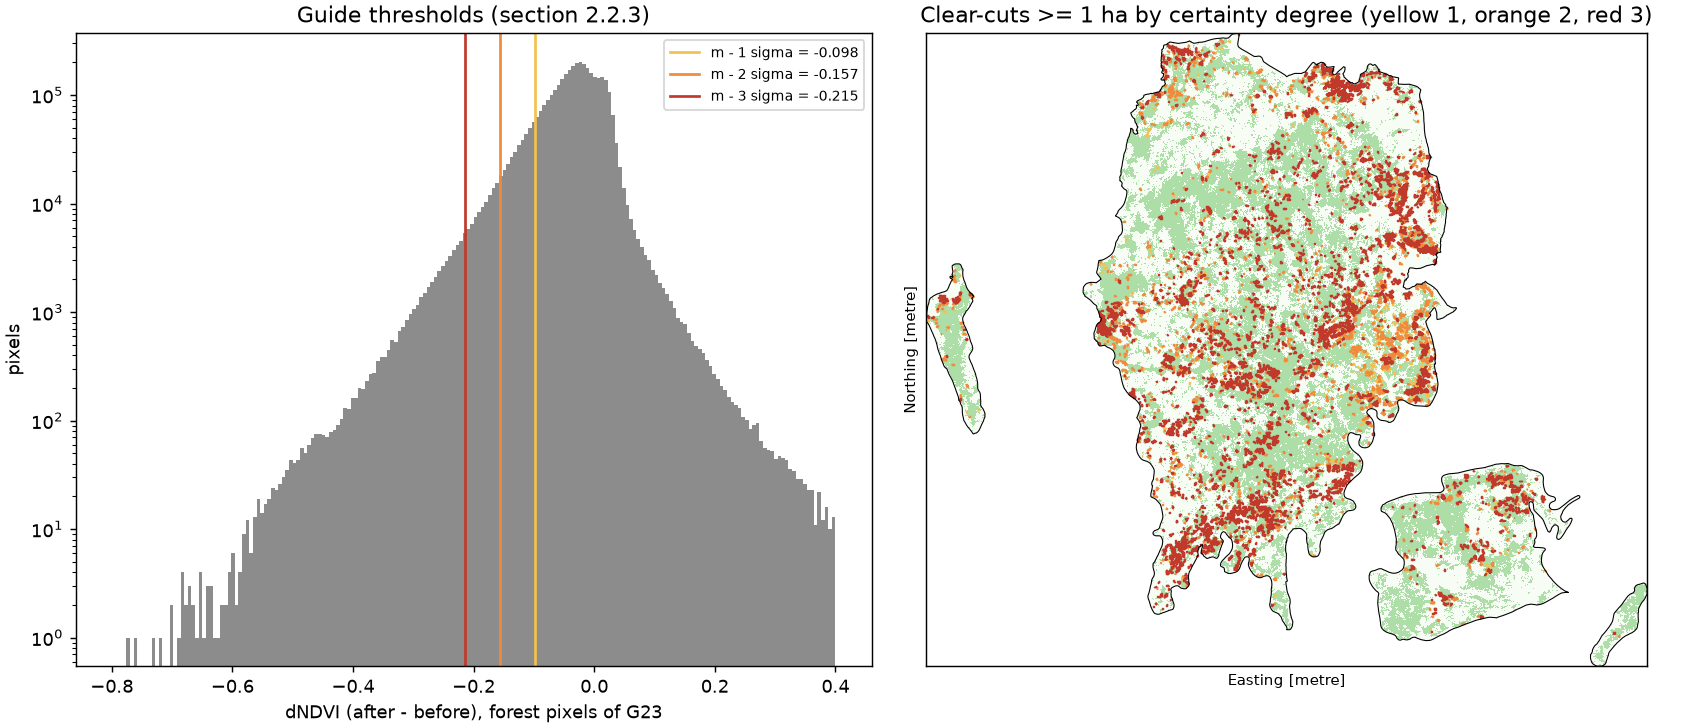
\includegraphics[width=0.9\linewidth]{s2_guide_overview.png}
\caption{Méthode du guide sur Sentinel-2, toute la G23 (degrés de certitude, juillet $\to$ septembre 2026).}
\label{fig-s2-overview}
\end{figure}

\paragraph{Référence qualifiée et photo-interprétation.} En ne gardant que le passage d'un état boisé au
sol nu (degré 3, NDVI avant $\geq 0{,}70$, après $\leq 0{,}65$, tamisage à 1~ha), on obtient 281 coupes
(613~ha). La photo-interprétation d'un échantillon de 30 coupes donne une précision de 59~\% (coupes
certaines) à 86~\% (avec les probables), sur 22 objets interprétables ; toutes les erreurs sont en
feuillus. Dans la fenêtre radar (\cref{fig-window}), les 60 coupes qualifiées ont toutes été examinées :
seules \textbf{10 montrent un sol nu certain} (1 en feuillus, 6 en résineux, 3 en mixtes), 9 sont
probables et 41 ne montrent pas de sol nu (sénescence, ombre, éclaircie). Le test \enquote{forêt avant}
(SWIR de juillet) écarte trois coupes déjà ouvertes en juillet. La référence principale compte donc
\textbf{7 coupes de peuplement fermé (15,4~ha)}.

\begin{figure}[H]
\centering
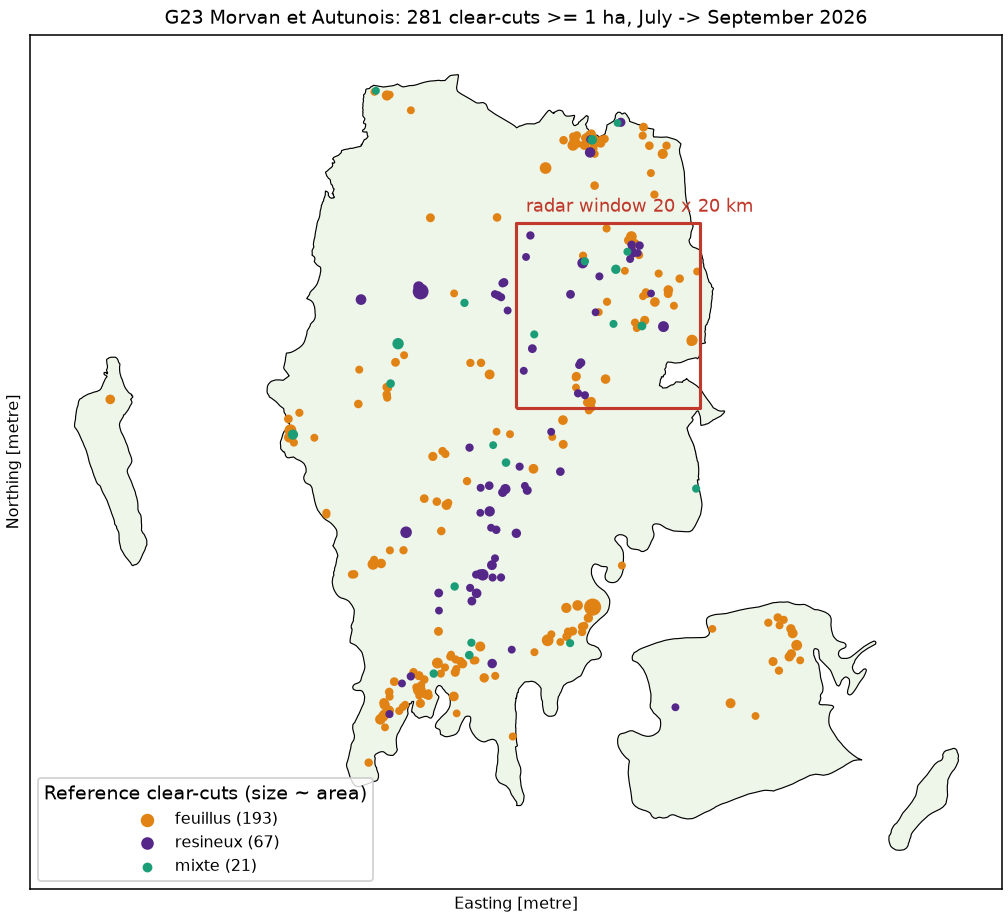
\includegraphics[width=0.8\linewidth]{s2_reference_window.png}
\caption{Fenêtre radar de $20\times20$~km et coupes de référence Sentinel-2.}
\label{fig-window}
\end{figure}

\subsection{Séparabilité coupe / forêt à géométrie égale}

Le \cref{tab-core} et la \cref{fig-summary} comparent les deux bandes à géométrie égale.

\begin{table}[H]
\centering\small
\caption{AUC coupe / forêt intacte [IC 95~\% par bootstrap en grappes], 7 coupes de peuplement.}
\label{tab-core}
\resizebox{\linewidth}{!}{\begin{tabular}{lcccc}
\toprule
Indicateur & L A173 & C A59 & L D66 & C D37 \\
\midrule
$\Delta\gamma^0$ pol. croisée & 0{,}80 {\scriptsize [0{,}61--0{,}93]} & 0{,}73 {\scriptsize [0{,}65--0{,}86]} & 0{,}83 {\scriptsize [0{,}66--0{,}93]} & 0{,}83 {\scriptsize [0{,}78--0{,}91]} \\
$\Delta\gamma^0$ co-pol. & 0{,}70 {\scriptsize [0{,}60--0{,}86]} & 0{,}63 {\scriptsize [0{,}53--0{,}77]} & 0{,}71 {\scriptsize [0{,}60--0{,}82]} & 0{,}74 {\scriptsize [0{,}67--0{,}82]} \\
$\gamma^0$ après, pol. croisée & 0{,}89 {\scriptsize [0{,}87--0{,}91]} & 0{,}76 {\scriptsize [0{,}72--0{,}84]} & 0{,}85 {\scriptsize [0{,}81--0{,}91]} & 0{,}82 {\scriptsize [0{,}75--0{,}89]} \\
cohérence minimale (co-pol.) & 0{,}60 {\scriptsize [0{,}53--0{,}66]} & 0{,}51 {\scriptsize [0{,}50--0{,}55]} & 0{,}81 {\scriptsize [0{,}75--0{,}86]} & 0{,}52 {\scriptsize [0{,}50--0{,}55]} \\
cohérence après (co-pol.) & 0{,}66 {\scriptsize [0{,}51--0{,}76]} & 0{,}68 {\scriptsize [0{,}61--0{,}79]} & 0{,}54 {\scriptsize [0{,}50--0{,}78]} & 0{,}74 {\scriptsize [0{,}66--0{,}83]} \\
\bottomrule
\end{tabular}
}
\end{table}

\begin{figure}[H]
\centering
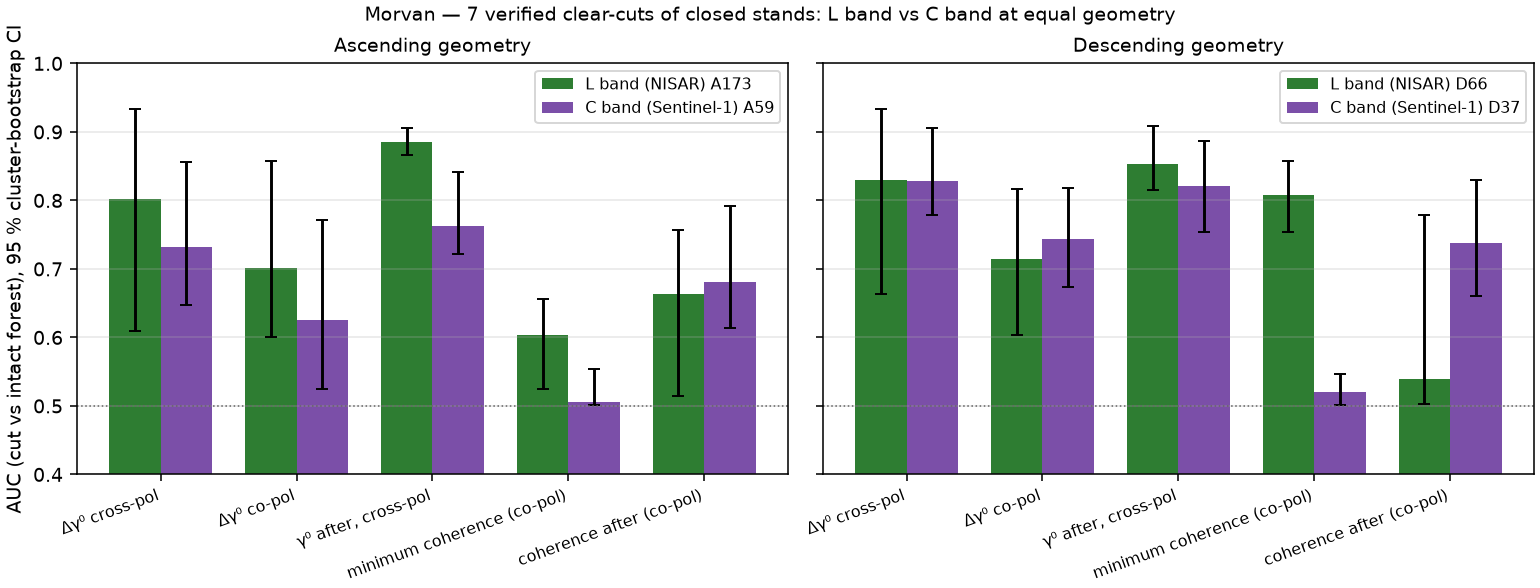
\includegraphics[width=\linewidth]{m8_summary_L_vs_C.png}
\caption{AUC des cinq indicateurs clés, bande L (vert) contre bande C (violet), en montante et en descendante.}
\label{fig-summary}
\end{figure}

\begin{table}[H]
\centering\small
\caption{Moyennes coupe / forêt intacte.}
\label{tab-means}
\begin{tabular}{lcccc}
\toprule
Coupe / forêt intacte & L A173 & C A59 & L D66 & C D37 \\
\midrule
$\Delta\gamma^0$ croisée (dB) & -2{,}49 / -0{,}23 & -1{,}76 / -0{,}44 & -2{,}66 / -0{,}33 & -2{,}59 / -0{,}60 \\
cohérence min. & 0{,}28 / 0{,}32 & 0{,}20 / 0{,}21 & 0{,}34 / 0{,}48 & 0{,}16 / 0{,}16 \\
\bottomrule
\end{tabular}

\end{table}

\begin{itemize}
\item \textbf{Rétrodiffusion croisée.} La baisse est plus forte en bande L ($-2{,}5$ et $-2{,}7$~dB contre
  $-1{,}8$ et $-2{,}6$~dB en C), et le d de Cohen est plus grand (1,89 et 2,13 contre 1,03 et 1,63). L'AUC
  est meilleure en L en montante (0,80 contre 0,73) et égale en descendante (0,83). Avec 7 coupes, les IC se
  recouvrent : aucune différence d'AUC en rétrodiffusion n'est significative.
\item \textbf{Polarisation.} La polarisation croisée sépare mieux que la co-polarisation dans les quatre
  géométries (H4).
\item \textbf{Contrôle avant coupe.} Les variables de changement restent près du hasard (AUC 0,50 à 0,57).
  Les variables de niveau avant la coupe atteignent 0,54 à 0,64 (0,70 à 0,75 avec la référence
  \enquote{vérifiée}) : les parcelles coupées sont des peuplements particuliers, surtout des résineux mûrs.
  Le $\gamma^0$ après la coupe (AUC 0,85 à 0,89) est donc en partie gonflé par le type de peuplement ;
  l'indicateur principal reste la variation $\Delta\gamma^0$.
\item \textbf{Pixels de bord.} Avec des objets érodés de 20~m, toutes les AUC augmentent de 0,03 à 0,07,
  sans changer l'ordre L / C.
\end{itemize}

\subsection{Cohérence interférométrique}

\begin{table}[H]
\centering\small
\caption{Cohérence médiane (co-polarisation) de la forêt intacte et des coupes après la coupe, sur l'ensemble
des paires à 12~jours (24~jours pour une paire NISAR par géométrie).}
\label{tab-coh}
\begin{tabular}{lcc}
\toprule
Géométrie & Forêt intacte & Coupes, après la coupe \\
\midrule
L A173 & 0,35 -- 0,70 & 0,41 -- 0,74 \\
L D66 & 0,48 -- 0,71 & 0,59 -- 0,71 \\
C A59 & 0,30 -- 0,36 & 0,34 -- 0,53 \\
C D37 & 0,25 -- 0,27 & 0,27 -- 0,38 \\
\bottomrule
\end{tabular}
\end{table}

En bande C, la forêt reste au plancher de l'estimateur (0,25 à 0,36 pour une fenêtre $10\times3$) : elle est
complètement décorrélée en 12 jours, comme dans les Vosges. En bande L, elle garde 0,5 à 0,7
(\cref{tab-coh}, H1). Une coupe y devient donc un événement : en D66, la cohérence minimale des coupes
tombe à 0,34 contre 0,48 pour la forêt (AUC 0,81 contre 0,52 en C D37). La paire du 29/08 au 10/09, qui
encadre trois coupes, donne 0,45 sur les coupes et 0,63 en forêt.

En montante (A173), l'avantage est faible (AUC 0,60) : deux paires de la fenêtre de coupe (13/08 $\to$
25/08 et 25/08 $\to$ 06/09) décorrèlent toute la forêt (0,35), probablement à cause d'un épisode de pluie
ou de vent, que nous n'avons pas vérifié. Enfin, en bande C, la coupe ne se voit qu'\emph{après} : le sol nu
redevient un peu cohérent en octobre--novembre (jusqu'à 0,53), alors que la forêt reste au plancher. D'où une
AUC de la cohérence après coupe plus élevée en C (0,68--0,74) qu'en L (0,54--0,66), mais 4 à 8 semaines
après la coupe.

\subsection{La méthode du guide transposée au radar}

\begin{table}[H]
\centering\small
\caption{Méthode du guide sur $\Delta\gamma^0$ croisée (meilleur degré par géométrie) : matrice de confusion
en surface, part des coupes trouvées (au moins 25~\% de leurs pixels) et fausses alertes en part de la forêt.}
\label{tab-guide}
\resizebox{\linewidth}{!}{\begin{tabular}{lllrrrcr}
\toprule
Géométrie & Variable & Degré & Omission (\%) & Commission (\%) & Kappa & Objets trouvés & Fausses alertes (\% forêt) \\
\midrule
L A173 & d\_g0\_HV & $\geq$2 & 55 & 62 & 0{,}41 & 5/7 & 0{,}09 \\
C A59 & d\_g0\_VH & $\geq$2 & 83 & 94 & 0{,}08 & 3/7 & 0{,}32 \\
L D66 & d\_g0\_HV & $\geq$2 & 51 & 64 & 0{,}41 & 5/7 & 0{,}10 \\
C D37 & d\_g0\_VH & $\geq$3 & 84 & 83 & 0{,}16 & 2/7 & 0{,}10 \\
\bottomrule
\end{tabular}
}
\end{table}

\begin{figure}[H]
\centering
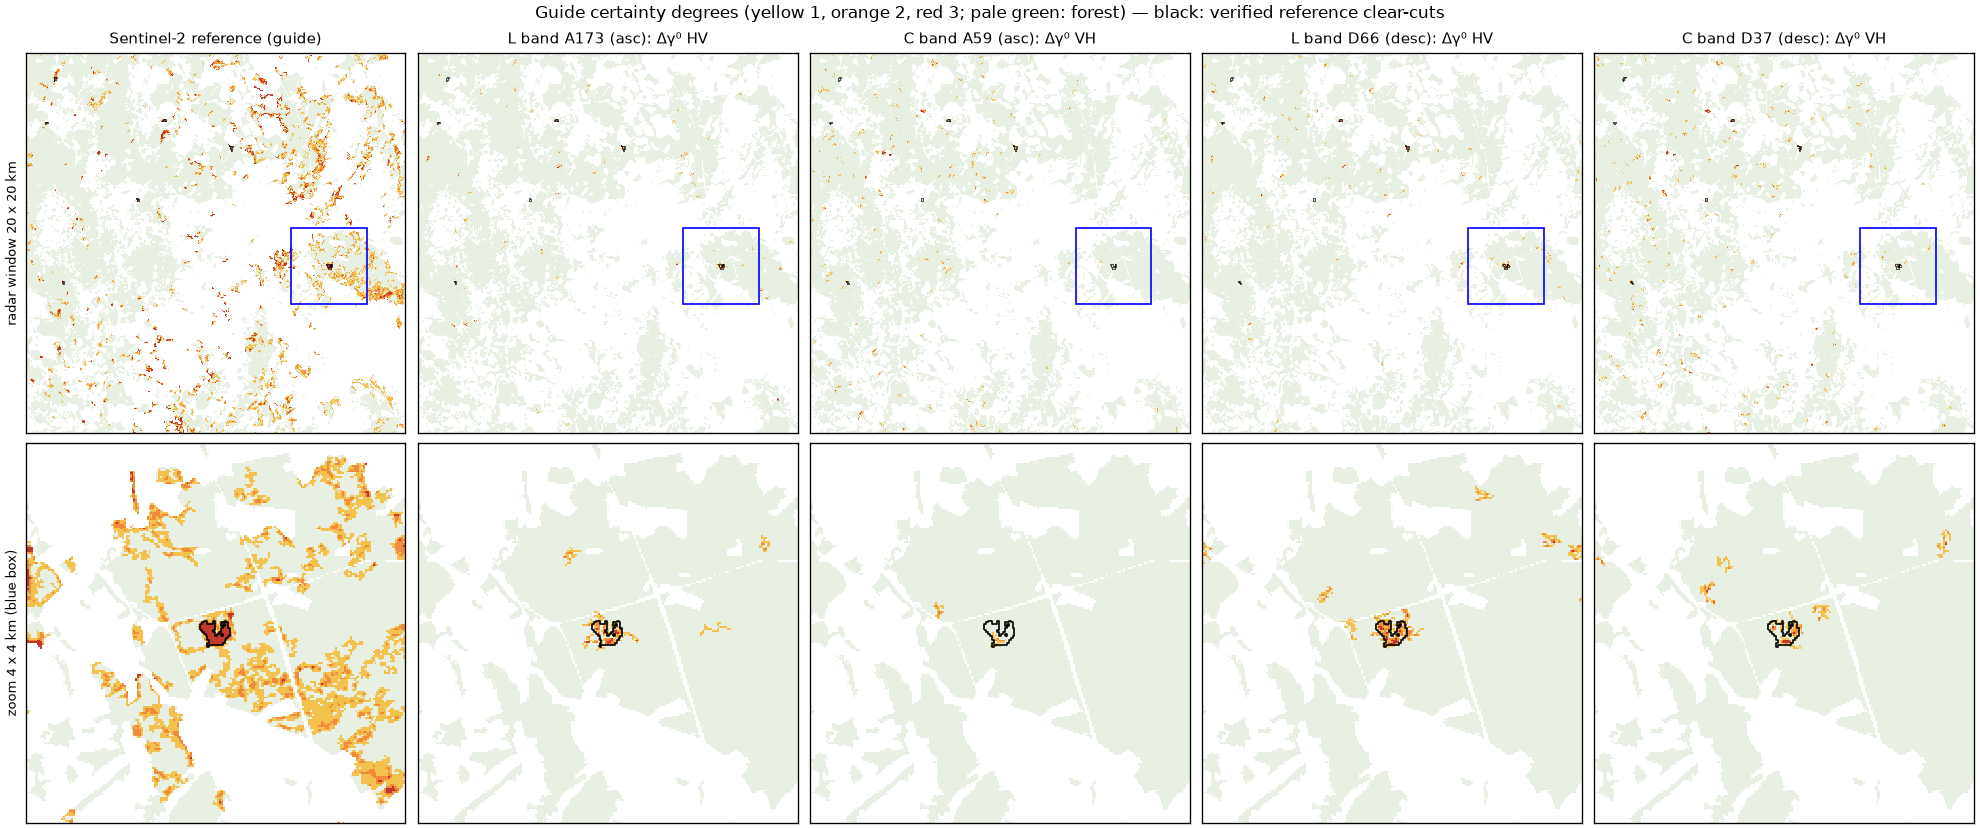
\includegraphics[width=\linewidth]{m6_guide_maps.png}
\caption{Degrés de certitude du guide (jaune 1, orange 2, rouge 3) : référence Sentinel-2, puis bande L et
bande C dans chaque direction. En haut, la fenêtre entière ; en bas, un zoom de $4\times4$~km (cadre bleu).
Contour noir : coupes de référence vérifiées.}
\label{fig-guide-maps}
\end{figure}

La bande L transpose bien mieux la méthode du guide : kappa 0,41 et 5 coupes sur 7 trouvées dans les deux
directions, contre un kappa de 0,08 à 0,16 et 2 à 3 coupes en bande C (\cref{tab-guide}, \cref{fig-guide-maps}).
Au même degré ($\geq 2$), la bande L produit 11 à 13~ha de fausses alertes sur 12\,800~ha évalués
(0,1~\% de la forêt), la bande C 41 à 52~ha. Ce résultat tient pour les quatre références (\cref{tab-refs-guide}).
On reste toutefois loin de l'objectif du guide (10~\% d'omission et de commission) : 51 à 55~\% d'omission et
62 à 64~\% de commission en L.

\begin{table}[H]
\centering\small
\caption{Kappa de la méthode du guide (meilleure combinaison) selon la référence.}
\label{tab-refs-guide}
\begin{tabular}{lcccc}
\toprule
Référence (objets) & L A173 & C A59 & L D66 & C D37 \\
\midrule
automatique (60) & 0,13 & 0,04 & 0,13 & 0,09 \\
vérifiées + probables (19) & 0,27 & 0,07 & 0,27 & 0,15 \\
vérifiées (10) & 0,34 & 0,08 & 0,34 & 0,19 \\
peuplement (7) & 0,41 & 0,08 & 0,41 & 0,16 \\
\bottomrule
\end{tabular}
\end{table}

\paragraph{Audit des fausses alertes.} Les 15 plus grands objets détectés par NISAR D66 hors de toute coupe
connue ont été photo-interprétés (\cref{fig-audit}). Deux sont des coupes tardives probables (F01, 2,5~ha ;
F04, 1,6~ha), coupées après la fenêtre \enquote{après} de Sentinel-2 ; les 13 autres sont des sénescences, des
lisières, des jaunissements de mélèze ou du bocage. Le même audit (\cref{fig-audit-s1}) sur Sentinel-1 D37 ($\Delta\gamma^0$ VH, degré 3, 15 plus grands objets) ne trouve \textbf{aucune coupe tardive} : 8 objets sur 15 (22~ha sur 36) sont des parcelles déjà ouvertes en juin (anciennes coupes, landes, prairies encore classées en forêt fermée par la BD Forêt), où la strate basse change (sénescence, travail du sol) ; les 7 autres sont des forêts intactes, des lisières ou des sénescences. La bande C réagit à la végétation basse, comme sur les coupes R019, R139 et R225 ouvertes avant juillet ; la bande L, non.

\begin{figure}[H]
\centering
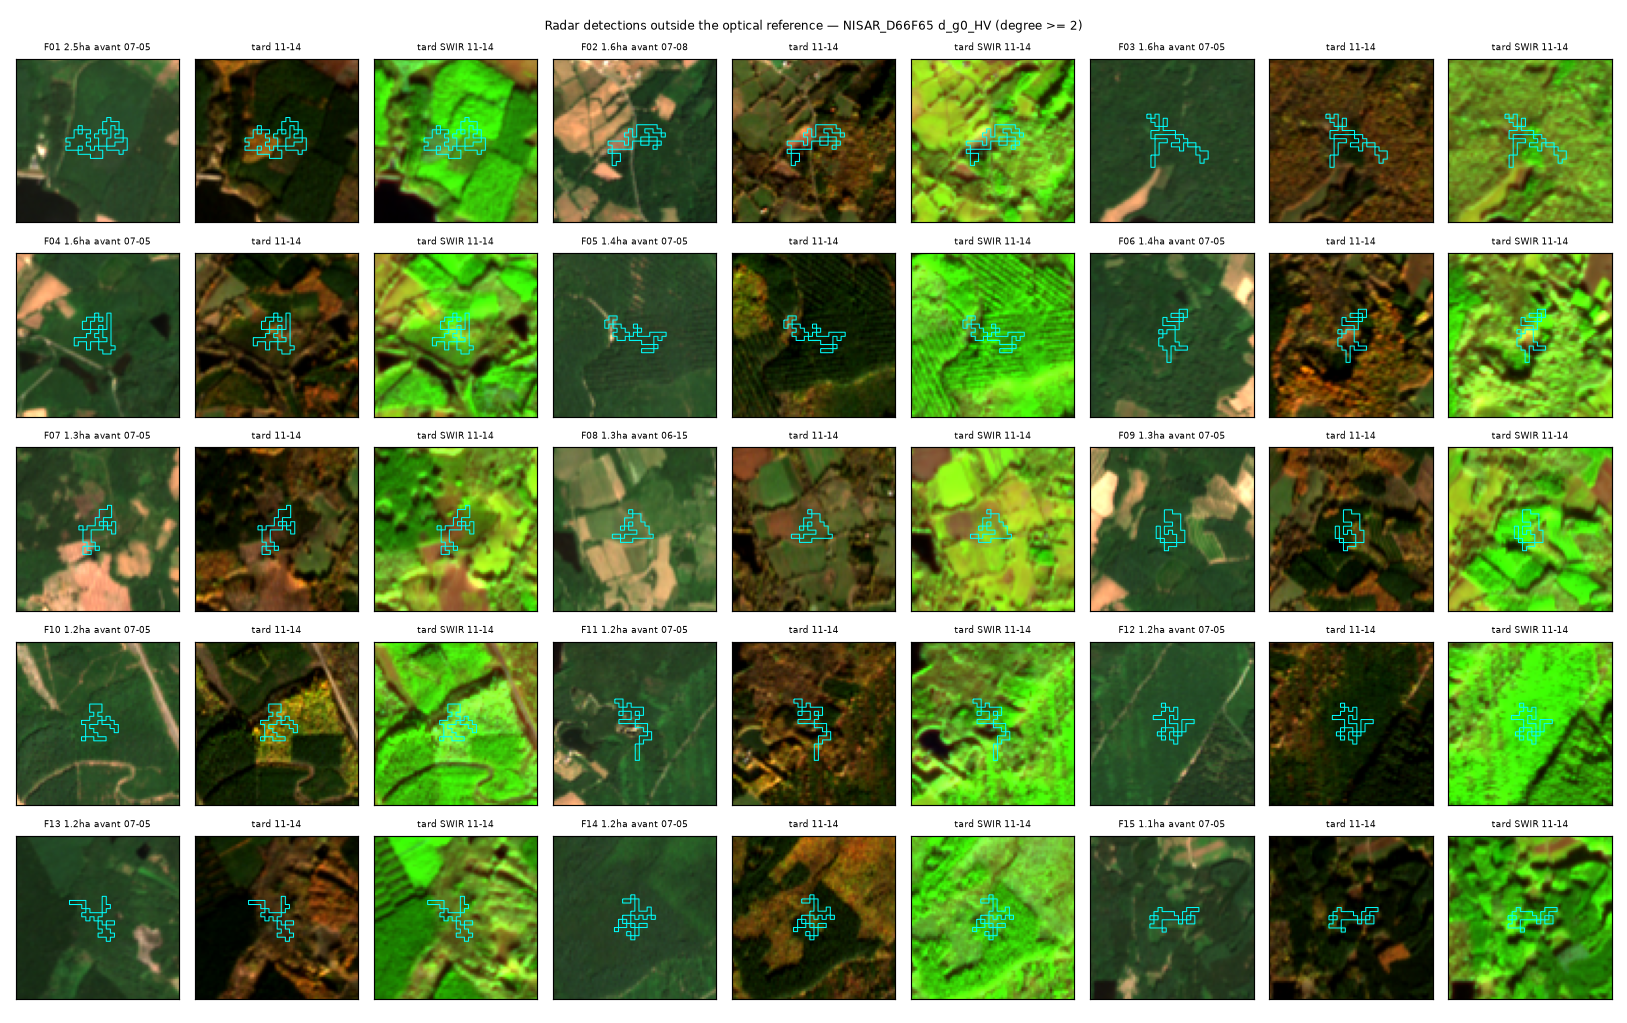
\includegraphics[width=\linewidth]{m6b_commission_NISAR_D66F65_d_g0_HV.png}
\caption{Audit des 15 plus grandes fausses alertes NISAR D66 : Sentinel-2 en juillet, en novembre (couleurs
vraies) et en novembre (SWIR / PIR / rouge).}
\label{fig-audit}
\end{figure}

\begin{figure}[H]
\centering
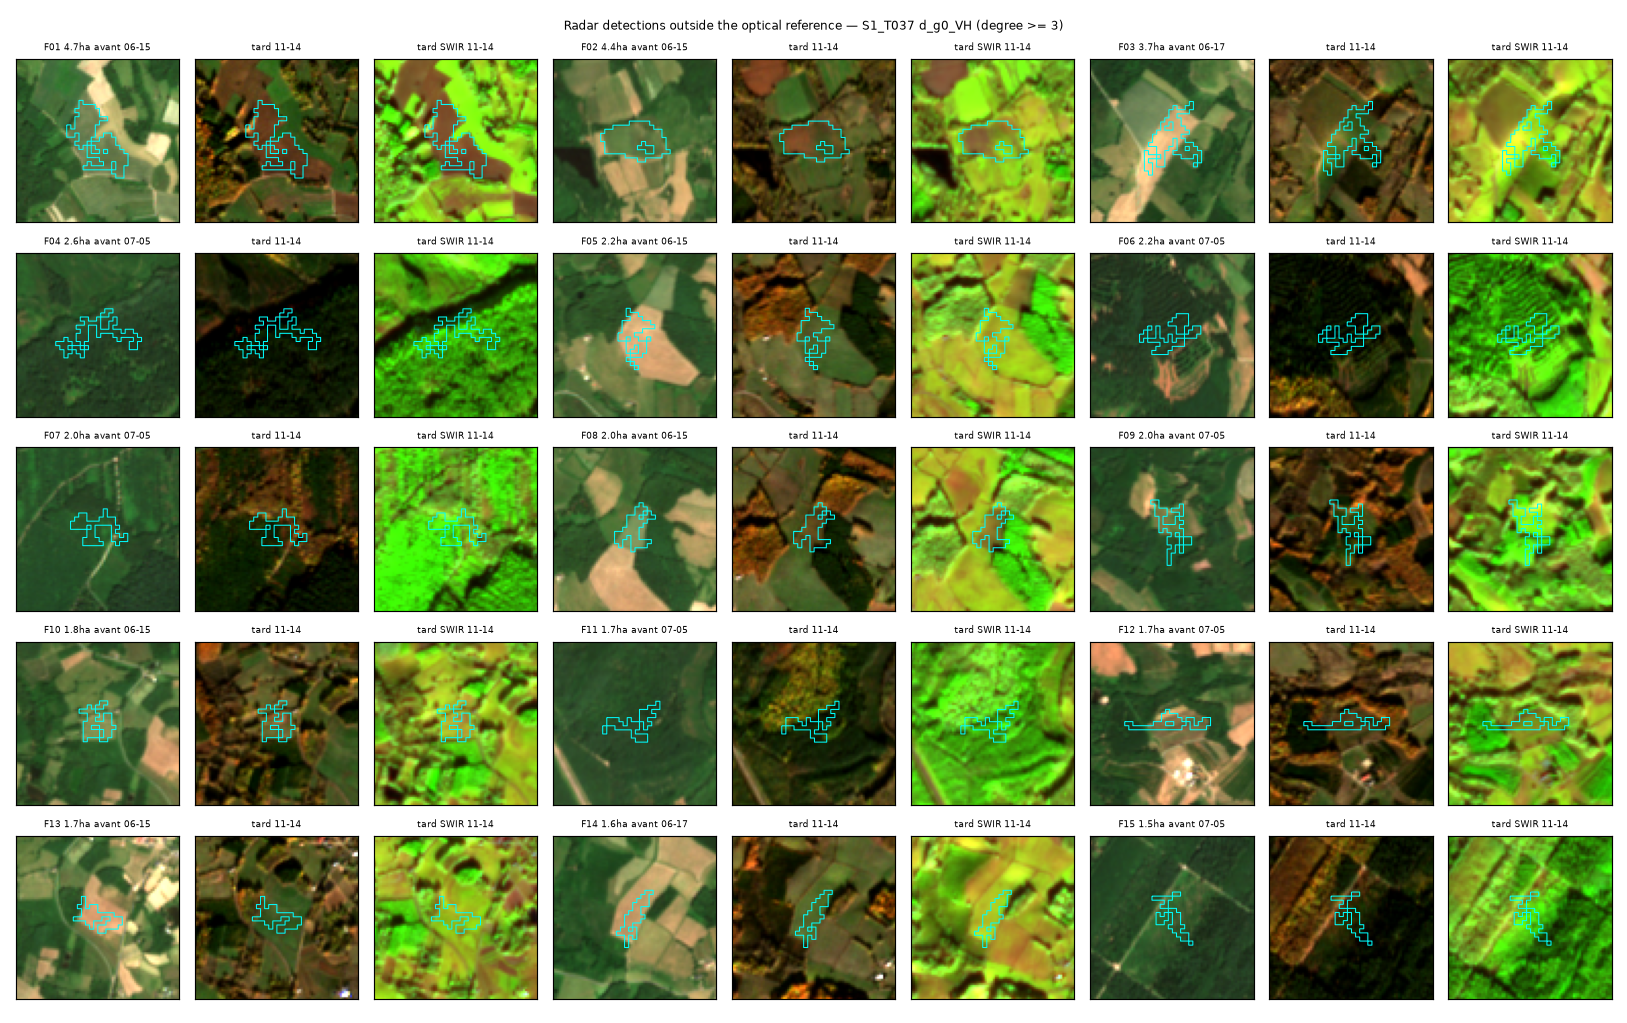
\includegraphics[width=\linewidth]{m6b_commission_S1_T037_d_g0_VH.png}
\caption{Audit des 15 plus grandes fausses alertes Sentinel-1 D37 (mêmes vignettes).}
\label{fig-audit-s1}
\end{figure}

\subsection{Sensibilité à la référence}

\begin{table}[H]
\centering\small
\caption{AUC de $\Delta\gamma^0$ croisée selon la référence.}
\label{tab-refs}
\begin{tabular}{lcccc}
\toprule
Référence (objets) & L A173 & C A59 & L D66 & C D37 \\
\midrule
auto (60) & 0{,}56 & 0{,}51 & 0{,}56 & 0{,}53 \\
vérifiées + probables (19) & 0{,}63 & 0{,}61 & 0{,}63 & 0{,}67 \\
vérifiées (10) & 0{,}68 & 0{,}70 & 0{,}71 & 0{,}78 \\
peuplement (7) & 0{,}80 & 0{,}73 & 0{,}83 & 0{,}83 \\
\bottomrule
\end{tabular}

\end{table}

La qualité de la référence domine tout le reste (\cref{tab-refs}) : l'AUC passe de 0,51--0,56 avec la
référence automatique à 0,73--0,83 avec les 7 coupes de peuplement. Sans photo-interprétation, on aurait
conclu à tort que ni la bande L ni la bande C ne voient les coupes. L'ordre L / C, lui, dépend de la
référence : avec les références \enquote{vérifiées}, la bande C égale ou dépasse la bande L (0,78 contre 0,71
en descendante). Ces références contiennent trois parcelles déjà ouvertes en juillet (R019, R139, R225) : leur
HV en bande L était déjà bas et baisse peu (moins de 1,3~dB), alors que la bande C, sensible à la végétation
basse et aux rémanents, baisse de 1,7 à 3,9~dB. La bande L répond à la perte des troncs, la bande C à tout
changement de la strate basse. C'est pourquoi la référence principale se limite aux peuplements fermés.

\subsection{Datation radar des coupes}

\begin{table}[H]
\centering\small
\caption{Intervalle de coupe (première baisse durable de plus de 2~dB en polarisation croisée), coupes
de peuplement fermé ; R : résineux, M : mixte, F : feuillus.}
\label{tab-dating}
\begin{tabular}{lcccc}
\toprule
Coupe & L A173 & C A59 & L D66 & C D37 \\
\midrule
R013 (R, 5{,}1 ha) & 25/08--06/09 & -- & 29/08--10/09 & 25/08--06/09 \\
R060 (M, 2{,}9 ha) & 25/08--06/09 & 09/07--21/07 & 29/08--10/09 & 25/08--06/09 \\
R100 (R, 2{,}1 ha) & -- & 07/09--19/09 & -- & 06/09--18/09 \\
R144 (R, 1{,}6 ha) & -- & -- & -- & 25/08--06/09 \\
R161 (F, 1{,}4 ha) & 06/09--18/09 & 07/09--19/09 & 29/08--10/09 & 06/09--18/09 \\
R198 (M, 1{,}3 ha) & 20/07--13/08 & 21/07--02/08 & 24/07--17/08 & 25/08--06/09 \\
R246 (R, 1{,}1 ha) & 20/07--13/08 & 14/08--26/08 & 12/07--24/07 & 25/08--06/09 \\
\bottomrule
\end{tabular}

\end{table}

\begin{figure}[H]
\centering
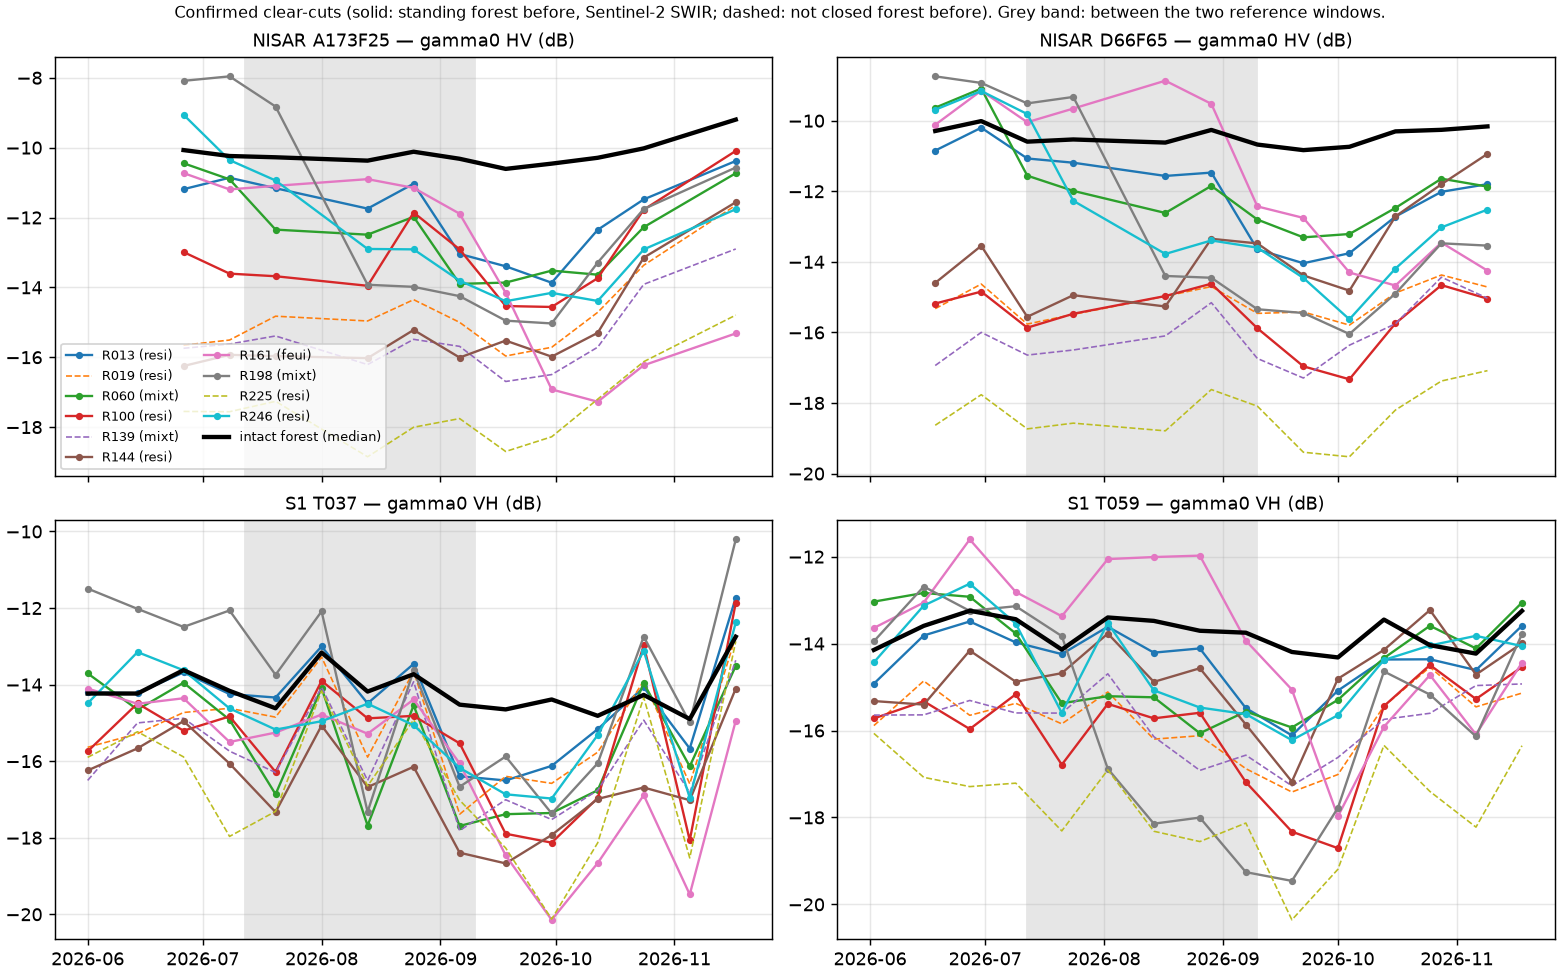
\includegraphics[width=\linewidth]{m7_cut_timeseries.png}
\caption{Séries de $\gamma^0$ en polarisation croisée des coupes confirmées et médiane de la forêt intacte.}
\label{fig-ts}
\end{figure}

En bande L, les séries sont lisses et les deux géométries concordent (\cref{tab-dating}, \cref{fig-ts}) :
R013 et R060 fin août -- début septembre, R161 début septembre, R198 et R246 fin juillet -- mi-août. En bande
C, l'orbite D37 subit des sauts synchrones de $\pm3$~dB sur toute la forêt, probablement liés à l'humidité ;
elle place 5 coupes sur 7 dans la même paire, ce qui n'est pas crédible. L'orbite A59, plus stable, resserre
la date de R198 (21/07 -- 02/08). R100 n'est détectée qu'en bande C (septembre, dans les deux orbites) ; en L,
la baisse reste sous 2~dB. Une éclaircie ou un débardage tardif, auquel la bande C réagit davantage, est
l'hypothèse la plus simple.

\subsection{Bilan des hypothèses}

\begin{table}[H]
\centering\small
\caption{Bilan des hypothèses sur le Morvan.}
\label{tab-hyp}
\begin{tabular}{lp{10.5cm}l}
\toprule
H & Constat & Verdict \\
\midrule
H1 & Forêt intacte : cohérence 0,5--0,7 en L contre 0,25--0,36 en C (plancher). & confirmée \\
H2 & D66 : AUC 0,81 contre 0,52 en C ; A173 : 0,60 (décorrélation générale fin août). & partielle \\
H3 & Baisse plus forte en L (d de Cohen 1,9--2,1 contre 1,0--1,6) ; AUC L $\geq$ C, non significatif. & partielle \\
H4 & Polarisation croisée $>$ co-polarisation dans les deux bandes et les quatre géométries. & confirmée \\
\bottomrule
\end{tabular}
\end{table}

%=====================================================================
\section{Discussion}

\paragraph{Comparaison avec les Vosges.} Les deux sites donnent le même message. La forêt reste cohérente
en bande L (0,64--0,70 dans les Vosges, 0,5--0,7 ici) et pas en bande C (0,28 et 0,25--0,36). L'avantage de
la bande L en rétrodiffusion dépend de la géométrie : dans les Vosges, il n'existait qu'en montante ; ici,
l'AUC est meilleure en montante et égale en descendante. La réplication lève les deux limites du premier
test (une seule coupe, une seule orbite Sentinel-1) et indique que le résultat des Vosges n'était pas
un cas isolé. En revanche, l'AUC de cohérence presque parfaite des Vosges (0,995) ne se retrouve pas : sur
7 coupes de dates différentes, les paires d'été sont parfois décorrélées sur toute la forêt.

\paragraph{Pourquoi la méthode du guide favorise la bande L.} À AUC égale (0,83 en descendante), la bande L
donne un kappa de 0,41 et la bande C de 0,16. L'AUC mesure le classement moyen des pixels ; une méthode à
seuils $m-k\sigma$ ne retient que la queue de la distribution, où compte l'écart exprimé en écarts-types
(d de Cohen 2,13 contre 1,63). La bande L est aussi plus stable d'une date à l'autre, ce qui resserre la
distribution de la forêt et réduit les fausses alertes. Pour un service opérationnel fondé sur des seuils,
c'est ce critère qui compte.

\paragraph{La référence, facteur limitant.} Le guide recommande le contrôle par photo-interprétation ; ce
travail montre qu'il est indispensable. En intra-saison, la sénescence des feuillus produit la plupart des
baisses de NDVI : seules 10 des 60 coupes qualifiées de la fenêtre sont des coupes certaines. Les scores
radar mesurés contre une référence automatique sont des bornes basses très pessimistes.

\paragraph{Complémentarité des deux bandes.} La bande C réagit à des événements que la bande L voit peu
(R100, sans doute une éclaircie ou un débardage) et sa revisite permet parfois de resserrer une date
(R198). La bande L donne des séries plus stables, des dates cohérentes entre géométries et moins de fausses
alertes. Un détecteur opérationnel gagnerait à combiner les deux, avec une confirmation temporelle.

\paragraph{Limites.} Sept coupes et 15~ha seulement : les IC sont larges et les différences d'AUC en
rétrodiffusion ne sont pas significatives. Une seule saison, un seul paysage dominé par les coupes de
résineux. La référence optique rate les coupes tardives (deux d'entre elles apparaissent comme fausses
alertes radar) et les coupes sans sol nu. Les estimateurs de cohérence diffèrent (NISAR GUNW contre SNAP
$10\times3$), les produits NISAR sont provisoires et la météo n'a pas été vérifiée.

%=====================================================================
\section{Conclusion}

Sur sept coupes rases vérifiées du Morvan et à géométrie égale dans les deux directions de visée :
\begin{enumerate}
\item la bande L garde la forêt cohérente (0,5--0,7) et la bande C non (plancher à 0,25--0,36) : H1 est
  confirmée sur un deuxième site ;
\item la cohérence L sépare les coupes en descendante (AUC 0,81 contre 0,52), moins en montante, où un
  épisode de décorrélation générale masque le signal ;
\item en rétrodiffusion, les AUC sont proches (L $\geq$ C), mais le contraste est plus fort en L, et la
  méthode du guide transposée au radar fonctionne bien mieux en bande L (kappa 0,41, 5 coupes sur 7) qu'en
  bande C (0,08--0,16, 2 à 3 coupes), sans atteindre l'objectif de 10~\% d'erreur ;
\item la qualité de la référence optique domine les résultats : la photo-interprétation est indispensable.
\end{enumerate}
La chaîne (paquet \texttt{nisar\_s1}, configuration par site) est directement transposable à ROSE-L~\cite{esa2020rosel}
et aux produits ISCE3~\cite{isce3}. La suite logique est un détecteur combinant cohérence L, rétrodiffusion L
et revisite C, évalué sur plusieurs saisons et plusieurs régions.


\printbibliography[heading=bibintoc,title={Références}]

\appendix
\section{Reproduction}
\begin{verbatim}
python morvan/scripts/m1_ign.py                 # contour G23, BD Forêt V2
python morvan/scripts/m2_s2_guide.py            # guide sur Sentinel-2, référence qualifiée
python morvan/scripts/m2b_photo_check.py        # photo-interprétation
python morvan/scripts/m2c_forest_before.py      # test « forêt avant » (SWIR)
python morvan/scripts/m3_radar_window.py        # choix de la fenêtre radar
python morvan/scripts/m4_fetch_nisar.py         # NISAR GCOV / GUNW (lecture à distance)
python morvan/scripts/m4_fetch_s1.py            # Sentinel-1 SLC réduits
python morvan/scripts/m5_process_s1.py --orbit 59   # SNAP (idem --orbit 37)
python morvan/scripts/m6_compare.py             # référence principale (peuplement)
python morvan/scripts/m6_compare.py --ref verifie --tag _verifie
python morvan/scripts/m6_compare.py --ref verifie_probable --tag _verifprob
python morvan/scripts/m6_compare.py --ref auto --tag _auto
python morvan/scripts/m6_compare.py --erode 20 --tag _erode20
python morvan/scripts/m6b_commission_audit.py --geom NISAR_D66F65 --var d_g0_HV
python morvan/scripts/m6b_commission_audit.py --geom S1_T037 --var d_g0_VH --degree 3
python morvan/scripts/m6c_coherence_pairs.py    # cohérence paire par paire
python morvan/scripts/m7_dating.py              # datation radar
python morvan/scripts/m8_make_tables.py         # tables LaTeX et figure de synthèse
\end{verbatim}

\section{Table complète de séparabilité}
\begin{table}[H]
\centering\scriptsize
\caption{Toutes les variables, référence principale (moyennes coupe / forêt, d de Cohen, AUC et IC 95~\%, distance de
Jeffries-Matusita).}
\begin{tabular}{llrrrrcr}
\toprule
Géométrie & Variable & Coupe & Forêt & d & AUC & IC 95 \% & JM \\
\midrule
L A173 & d\_g0\_HH & -0{,}91 & 0{,}33 & -1{,}02 & 0{,}70 & 0{,}60--0{,}86 & 0{,}25 \\
L A173 & g0\_post\_HH & -7{,}00 & -5{,}18 & -0{,}89 & 0{,}76 & 0{,}70--0{,}83 & 0{,}19 \\
L A173 & d\_g0\_HV & -2{,}49 & -0{,}23 & -1{,}89 & 0{,}80 & 0{,}61--0{,}93 & 0{,}51 \\
L A173 & g0\_post\_HV & -13{,}94 & -10{,}54 & -1{,}52 & 0{,}89 & 0{,}87--0{,}91 & 0{,}57 \\
L A173 & coh\_min\_HH & 0{,}28 & 0{,}32 & -0{,}37 & 0{,}60 & 0{,}53--0{,}66 & 0{,}07 \\
L A173 & coh\_drop\_HH & 0{,}33 & 0{,}29 & 0{,}27 & 0{,}58 & 0{,}50--0{,}74 & 0{,}02 \\
L A173 & coh\_post\_HH & 0{,}54 & 0{,}49 & 0{,}52 & 0{,}66 & 0{,}51--0{,}76 & 0{,}08 \\
L D66 & d\_g0\_HH & -0{,}99 & 0{,}20 & -1{,}10 & 0{,}71 & 0{,}60--0{,}82 & 0{,}26 \\
L D66 & g0\_post\_HH & -7{,}04 & -5{,}53 & -0{,}79 & 0{,}72 & 0{,}66--0{,}83 & 0{,}15 \\
L D66 & d\_g0\_HV & -2{,}66 & -0{,}33 & -2{,}13 & 0{,}83 & 0{,}66--0{,}93 & 0{,}57 \\
L D66 & g0\_post\_HV & -13{,}82 & -10{,}72 & -1{,}43 & 0{,}85 & 0{,}81--0{,}91 & 0{,}45 \\
L D66 & coh\_min\_HH & 0{,}34 & 0{,}48 & -1{,}17 & 0{,}81 & 0{,}75--0{,}86 & 0{,}36 \\
L D66 & coh\_drop\_HH & 0{,}10 & 0{,}02 & 0{,}74 & 0{,}68 & 0{,}60--0{,}79 & 0{,}13 \\
L D66 & coh\_post\_HH & 0{,}60 & 0{,}62 & -0{,}16 & 0{,}54 & 0{,}50--0{,}78 & 0{,}01 \\
C D37 & d\_g0\_VH & -2{,}59 & -0{,}60 & -1{,}63 & 0{,}83 & 0{,}78--0{,}91 & 0{,}44 \\
C D37 & g0\_post\_VH & -16{,}76 & -14{,}55 & -1{,}27 & 0{,}82 & 0{,}75--0{,}89 & 0{,}35 \\
C D37 & d\_g0\_VV & -1{,}88 & -0{,}52 & -1{,}16 & 0{,}74 & 0{,}67--0{,}82 & 0{,}27 \\
C D37 & g0\_post\_VV & -10{,}09 & -8{,}35 & -1{,}04 & 0{,}78 & 0{,}69--0{,}85 & 0{,}24 \\
C D37 & coh\_min\_VH & 0{,}14 & 0{,}15 & -0{,}21 & 0{,}56 & 0{,}54--0{,}60 & 0{,}02 \\
C D37 & coh\_drop\_VH & 0{,}11 & 0{,}11 & 0{,}08 & 0{,}53 & 0{,}50--0{,}56 & 0{,}01 \\
C D37 & coh\_post\_VH & 0{,}31 & 0{,}26 & 0{,}74 & 0{,}69 & 0{,}64--0{,}77 & 0{,}12 \\
C D37 & coh\_min\_VV & 0{,}16 & 0{,}16 & 0{,}04 & 0{,}52 & 0{,}50--0{,}55 & 0{,}01 \\
C D37 & coh\_drop\_VV & 0{,}11 & 0{,}11 & -0{,}02 & 0{,}50 & 0{,}50--0{,}55 & 0{,}00 \\
C D37 & coh\_post\_VV & 0{,}35 & 0{,}27 & 1{,}12 & 0{,}74 & 0{,}66--0{,}83 & 0{,}26 \\
C A59 & d\_g0\_VH & -1{,}76 & -0{,}44 & -1{,}03 & 0{,}73 & 0{,}65--0{,}86 & 0{,}22 \\
C A59 & g0\_post\_VH & -15{,}54 & -13{,}86 & -1{,}01 & 0{,}76 & 0{,}72--0{,}84 & 0{,}23 \\
C A59 & d\_g0\_VV & -1{,}11 & -0{,}34 & -0{,}62 & 0{,}63 & 0{,}53--0{,}77 & 0{,}15 \\
C A59 & g0\_post\_VV & -9{,}30 & -8{,}01 & -0{,}80 & 0{,}72 & 0{,}68--0{,}79 & 0{,}14 \\
C A59 & coh\_min\_VH & 0{,}19 & 0{,}20 & -0{,}12 & 0{,}53 & 0{,}50--0{,}56 & 0{,}01 \\
C A59 & coh\_drop\_VH & 0{,}10 & 0{,}10 & -0{,}05 & 0{,}52 & 0{,}50--0{,}57 & 0{,}00 \\
C A59 & coh\_post\_VH & 0{,}33 & 0{,}32 & 0{,}24 & 0{,}57 & 0{,}53--0{,}62 & 0{,}02 \\
C A59 & coh\_min\_VV & 0{,}20 & 0{,}21 & -0{,}06 & 0{,}51 & 0{,}50--0{,}55 & 0{,}01 \\
C A59 & coh\_drop\_VV & 0{,}11 & 0{,}11 & 0{,}02 & 0{,}51 & 0{,}50--0{,}54 & 0{,}00 \\
C A59 & coh\_post\_VV & 0{,}38 & 0{,}33 & 0{,}73 & 0{,}68 & 0{,}61--0{,}79 & 0{,}12 \\
\bottomrule
\end{tabular}

\end{table}

\section{Séparabilité par groupe forestier}
\begin{table}[H]
\centering\small
\caption{AUC de $\Delta\gamma^0$ croisée par groupe forestier, référence automatique (60 objets). Les valeurs proches de
0,5 en feuillus traduisent surtout les erreurs de la référence (sénescence).}
\begin{tabular}{lcccc}
\toprule
Groupe (pixels coupe) & L A173 & C A59 & L D66 & C D37 \\
\midrule
feuillus (1560) & 0{,}52 & 0{,}56 & 0{,}53 & 0{,}54 \\
résineux (959) & 0{,}55 & 0{,}52 & 0{,}58 & 0{,}59 \\
mixtes (279) & 0{,}74 & 0{,}67 & 0{,}70 & 0{,}70 \\
\bottomrule
\end{tabular}

\end{table}

\end{document}
